\begin{figure}[t]
  \centering
  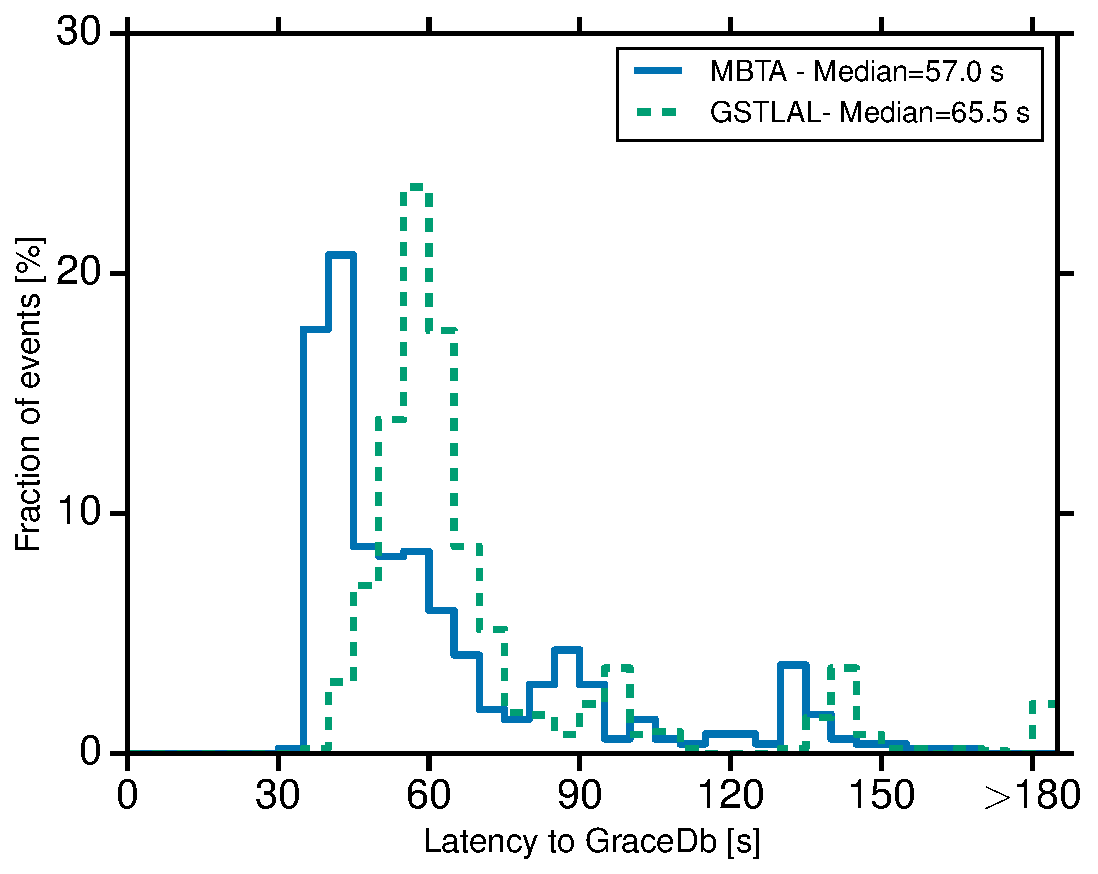
\includegraphics[width=0.45\textwidth]{figure2}
  \caption{\label{fig:latency} Latency of the online searches during O1.
           The latency is measured as the time between the event arriving at Earth
           and time at which the event is uploaded to \ac{GraCEDb}.}
\end{figure}

The offline search, targeting \ac{BBH} as well as \ac{BNS} and \ac{NSBH} mergers, identified
two signals with $> 5 \sigma$ confidence in the \ac{O1} dataset~\citep{Abbott:2016blz,Abbott:2016nmj}. A third signal was
also identified with \LVBLAHsignificance\ confidence~\citep{TheLIGOScientific:2016pea, TheLIGOScientific:2016qqj}. Subsequent
parameter inference on all three of these events has determined that, to very high
confidence, they were not produced by a \ac{BNS} or \ac{NSBH} merger~\citep{TheLIGOScientific:2016wfe, TheLIGOScientific:2016pea}. No other events
are significant with respect to the noise background in the offline search~\citep{TheLIGOScientific:2016pea}, and
we therefore state that no \ac{BNS} or \ac{NSBH} mergers were observed.

The online search identified a total of \OoneOnlineTotalEMFollowUpEvents\ unique \ac{GW} candidate events
with a false-alarm rate (FAR) less than
$6\, \mathrm{yr}^{-1}$.
Events with a FAR less than this are sent to electromagnetic partners if they
pass event validation.
Six of the events were rejected during the event validation as they were associated
with known non-Gaussian behavior in one of the observatories. Of the remaining
events, one was the \ac{BBH} merger GW151226 reported in~\citep{Abbott:2016nmj}. The second
event identified by \gstlal\ was only narrowly below the FAR threshold, with a FAR of $3.1\, \mathrm{yr}^{-1}$.
This event was also detected by \mbta\ with a higher FAR of $35\, \mathrm{yr}^{-1}$.
This is consistent with noise in the online searches and the candidate event was later
identified to have a false alarm rate of $190\, \mathrm{yr}^{-1}$
in the offline \gstlal\ analysis.
Nevertheless, the event passed all event validation and was released for \ac{EM} follow-up observations,
which showed no significant counterpart. The results
of the \ac{EM} follow-up program are discussed in more detail in~\citep{Abbott:2016gcq}.

All events identified by the \gstlal\ or \mbta\ online analyses with a false alarm rate of less than
$3200 \, \mathrm{yr}^{-1}$
are uploaded to an internal database known
as the \acf{GraCEDb}~\citep{gracedb}.
In total \OoneOnlineTotalMBTAGraceDBEvents\ events were uploaded from \mbta\
and \OoneOnlineTotalGSTLALGraceDBEvents\ from \gstlal.
We can measure the latency of the online pipelines from the time between the
inferred arrival time of each event at the Earth and the time at which the
event is uploaded to \ac{GraCEDb}. This latency is illustrated in Fig.~\ref{fig:latency},
where it can be seen that both online pipelines acheived median latencies on
the order of one minute. We note that \gstlal\ uploaded twice as many events as \mbta\
because of a difference in how the FAR was defined. The FAR reported by \mbta\ was defined
relative to the rate of coincident data such that an event with a FAR of $1 \, \mathrm{yr}^{-1}$
is expected to occur once in a year of coincident data. The FAR reported by \gstlal\ was defined 
relative to wall-clock time such that an event with a FAR of $1 \, \mathrm{yr}^{-1}$
is expected to occur once in a calendar year. In the following section we use the \mbta\
definition of FAR when computing rate upper limits.